\chapter{Opis sustava i tehničkih zahtjeva}

\section{Moderna poljoprivreda}

%Moj problematični poljoprivredni sustav. Ovdje opisati sa čim se poljopvrivrednici bore, šta im smeta, potkrijepiti to tako linkovima, onda naći rješenja koja su im pomogla i kako im IoT poljoprivreda boosta productivity i poboljšava usjeve i tako to. 

\section{Zahtjevi na sustav i opis predloženog rješenja}

Sustav za udaljeni nadzor u poljoprivredi treba omogućiti praćenje parametara poljoprivredne površine u stvarnom vremenu. Da bi se to postiglo, potrebno je na površinu postaviti uređaj s primjerenim senzorima te omogućiti bežično slanje očitanih senzorskih mjerenja u stvarnom vremenu u računalni oblak. Odabrana je arhitektura gdje se mikrokontrolerski razvojni sustav s priključenim senzorima koristi za mjerenje parametara, a putem ugrađene podrške za bežično povezivanje na Wi-Fi šalje podatke prema oblaku. Isto tako, odabran je računalni oblak koji nudi obradu podataka i njihovu trajnu pohranu te vizualizaciju. 

Prilikom odabira razvojnog sustava potrebno je paziti da ima mogućnost bežičnog povezivanja putem Wi-Fi mreže. Također je važno odabrati prikladan skup senzora koji prate uvjete nužne za održavanje poljoprivredne površine. Za računalni oblak potrebno je odabrati platformu koja može progutati i obraditi veliku količinu podataka te ih zatim pohraniti. Isto tako, potrebno je omogućiti jednostavno uspostavljanje komunikacije između mikrokontrolerskog razvojnog sustava i odabrane platforme. U oblaku je također bilo potrebno izraditi web aplikaciju koja mora korisniku pružiti jednostavnu vizualizaciju pohranjenih podataka. Glavna uloga aplikacije jest prikazati podatke i tako korisniku omogućiti udaljeno praćenje poljoprivrednih uvjeta kroz vrijeme. 

Za potrebe ovog rada odabran je razvojni sustav ESP32-C3-DevKitM-1 jer zadovoljava postavljene zahtjeve i ima mogućnost jednostavnog razvoja programske potpore korištenjem ugrađenih biblioteka. Na razvojnom sustavu nalazi se modul ESP32-C3 koji ima ugrađeno sučelje za povezivanje putem Wi-Fi mreže. Kao računalna platforma u oblaku odabran je sustav Amazon Web Services (AWS) jer nudi lako skalabilnu obradu podataka, kao i baze za njihovu pohranu. Za web aplikaciju odabrana je višeplatformska aplikacija Grafana koja pruža različite vrste vizualizacija, čime se poboljšava korisničko iskustvo pregleda podataka. Aplikacija također podržava alarmiranje korisnika o neželjenim uvjetima. Blok shema sustava prikazana je na slici \ref{fig:shema}. U nastavku rada opisani su svi aspekti programskog rješenja razvijeni u okviru rada, odnosno programska potpora za mikrokontrolerski sustav, kao i potpora za oblak.

\begin{figure}[ht]
	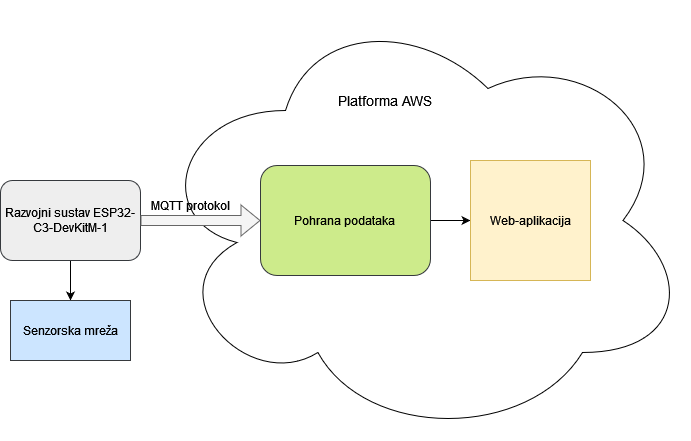
\includegraphics[width=\linewidth]{imgs/shema}
	\caption{Blok shema sustava}
	\label{fig:shema}
\end{figure}

